\documentclass[fullscreen=true, bookmarks=true, hyperref={pdfencoding=unicode}]{beamer}
\usepackage[utf8]{inputenc}                                % Кодировка
\usepackage[english,russian]{babel}                        % Переносы
\usepackage{xcolor}                                        % Работа с цветом
\usepackage{amsmath,amssymb,amsfonts}                      % Символы АМО
\usepackage{graphicx}                                      % Графика
\usepackage[labelsep=period]{caption}                      % Разделитель в подписях к рисункам и таблицам
\usepackage{hhline}                                        % Для верстки линий в таблицах
\usepackage{tikz}                                          % Для простых рисунков в документе
\usepackage{fancybox}                                      % Пакет для отрисовки рамок
\usepackage{verbatim}                                      % Для вставки кода в презентацию
\usepackage{animate}                                       % Для вставки видео в презентацию
\usepackage{xmpmulti}                                      % Для вставки gif в презентацию
\usepackage{multirow}
\usepackage{mathrsfs}

\usetikzlibrary{arrows, snakes, backgrounds}                 % Для отрисовки стрелок
\usetikzlibrary{positioning, fit, arrows.meta, shapes, calc}
% used to avoid putting the same thing several times...
% Command \empt{var1}{var2}
\newcommand{\empt}[2]{$#1^{\langle #2 \rangle}$}

\graphicspath{{images/}}                                   % Путь до рисунков
\setbeamertemplate{caption}[numbered]                      % Включение нумерации рисунков

\definecolor{links}{HTML}{2A1B81}                          % blue for url links
\hypersetup{colorlinks,linkcolor=,urlcolor=links}          % nothing for others

\usetheme{Boadilla}
\usecolortheme{whale}

\usepackage{minted}

% \setbeameroption{show notes}
% \setbeameroption{hide notes}
\setbeameroption{show only notes}

\title{Lecture 10. Attention Models and Transformers}
\author{Alex Avdyushenko}
\institute{Kazakh-British Technical University}
\date{November 12, 2022}
\titlegraphic{
\includegraphics[keepaspectratio,width=0.4\textwidth]{logo_kbtu.png}}


\begin{document}
%\unitlength=2mm

% выводим заглавие
\begin{frame}
\transdissolve[duration=0.2]
\titlepage
\end{frame}

\note{Good afternoon, dear students. Today we are going to talk about attention and transformers — probably the most breakthrough architecture of the last maybe five years of deep learning. This is a very interesting approach, and again it is quite similar to human information processing.}

\begin{frame}
  \frametitle{Five-minutes block}
  \pause
  \begin{itemize}
     \item List the disadvantages of convolutional neural networks
     \item Write the formula for the simplest (vanilla) recurrent network module
     \item What kind of filters (gates) does LSTM have?
  \end{itemize}
\end{frame}

\note{Ok, great, and as always we start with traditional five-minutes questions on the previous lecture. Please, write answers or send photos with them directly to me in private messages here in Teams or may be in Telegram, but choose only one option please :)}

\begin{frame}[t]
  \frametitle{Disadvantages of vanilla Recurrent Neural Network}
  \framesubtitle{Recall}

  We use one hidden vector
  $$ h_t = f_W(h_{t-1}, x_t)$$

  As a function $f_W$ we set a linear transformation with a non-linear component-wise "sigmoid":

  \begin{align*}
    h_t &= \tanh ({\color{red}W_{hh}} h_{t-1} + {\color{red}W_{xh}} x_t) \\
    y_t &= {\color{red}W_{hy}} h_t
  \end{align*}

  \pause
  Disadvantages
   \begin{enumerate}
     \item input and output sequence lengths must match
     \item ``reads'' the input only from left to right, does not look ahead
     \item therefore it is not suitable for machine translation, question answering tasks and others
   \end{enumerate}

\end{frame}

\note{Now, let's remember vanilla recurrent neural network and it's disadvantages.}

\begin{frame}
  \frametitle{RNN for sequence synthesis (seq2seq)}
  \framesubtitle{Recall}

  $X = (x_1, \dots, x_n)$ — input sequence

  $Y = (y_1, \dots, y_m)$ — output sequence

  ${\color{red}c \equiv h_n}$ encodes all information about $X$ to synthesize $Y$

  \begin{center}
    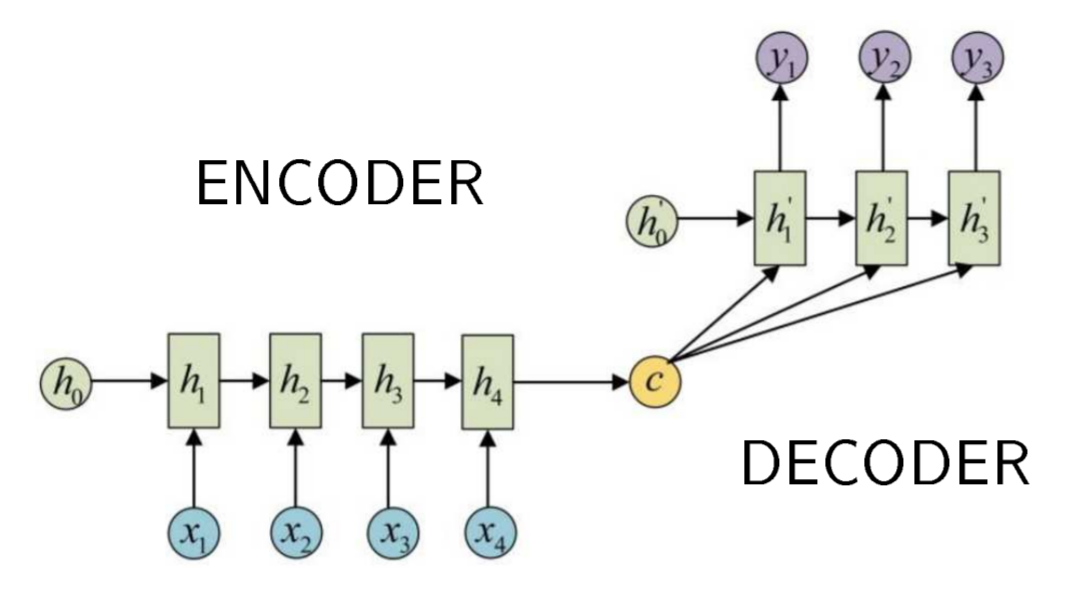
\includegraphics[keepaspectratio,
                     width=.5\paperwidth]{seq2seq.png}
   \end{center}

  \begin{center}
    \begin{align*}
      h_i &= f_{in}(x_i, h_{i-1}) \\
      {\color{red}h_t^\prime} &{\color{red}= f_{out}(h_{t-1}^\prime,y_{t-1},c)} \\
      y_t &= f_{y}(h_t^\prime, y_{t-1})
    \end{align*}
  \end{center}
\end{frame}

\note{Ok, next step. How can we solve this problems? For example, we can use seq2seq architecture.}

\begin{frame}
  \begin{center}
    \begin{align*}
      h_i &= f_{in}(x_i, h_{i-1}) \\
      {\color{red}h_t^\prime} &{\color{red}= f_{out}(h_{t-1}^\prime,y_{t-1},c)} \\
      y_t &= f_{y}(h_t^\prime, y_{t-1})
    \end{align*}
  \end{center}

  \pause
  Disadvantages
    \begin{itemize}
      \item $c$ remembers the end ($h_n$) better than the start
      \item the more $n$, the more difficult to pack all the information into vector $c$
      \item we should control the vanishing and explosions of the gradient
      \item RNN is difficult to parallelize
    \end{itemize}
    \pause
    \begin{block}{Question}
      How can you fix some of the problems above?
    \end{block}
    \pause
    \begin{exampleblock}{Hint}
      How do people perceive information?
    \end{exampleblock}
\end{frame}

\note{Now, as is often the case  we have new, more difficult problems with seq2seq architecture.}

\begin{frame}
  \frametitle{Let's count the number of passes}

  \begin{center}
    \href{https://www.youtube.com/watch?v=vJG698U2Mvo}{Basketball!}
  \end{center}
\end{frame}

\note{Now let's have some fun and count the number of passes in the video.}

\begin{frame}
  \frametitle{RNN with attention mechanism}

   $a(h, h^\prime)$ is the similarity function of input $h$ and output $h^\prime$
   (for example, dot product or $\exp(h^T h^\prime)$ and others)

   \vspace{0.5cm}
   $\alpha_{ti}$ — importance of input $i$ for output $t$ (attention score), $\sum\limits_i \alpha_{ti} = 1$

   $c_t$ — input context vector for output $t$
  \begin{center}
    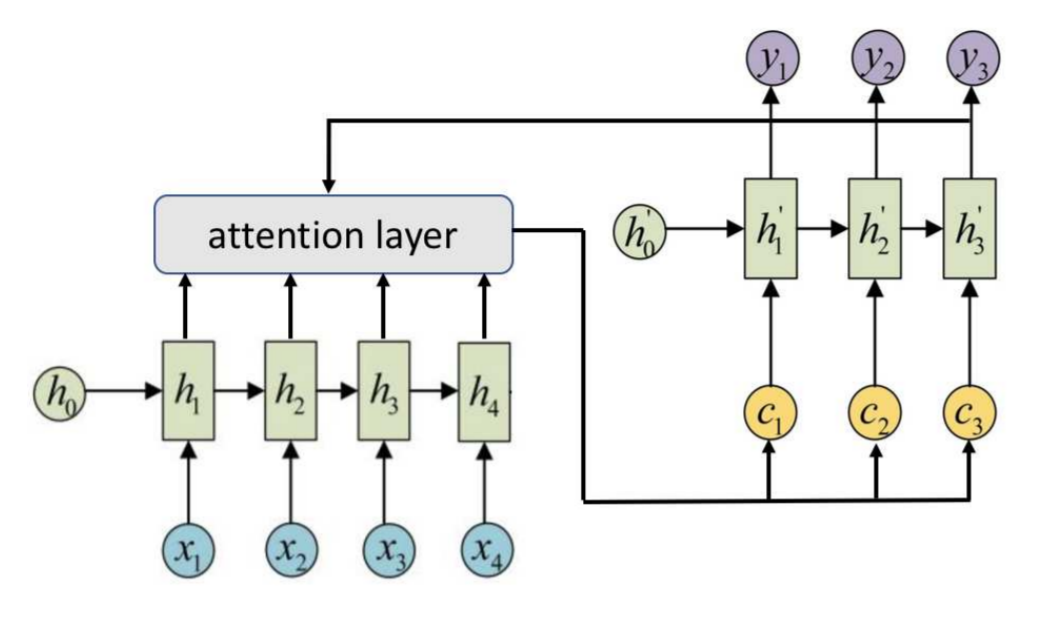
\includegraphics[keepaspectratio,
                   width=.6\paperwidth]{seq2seq_attention.png}
  \end{center}
\end{frame}

\note{So, how can we use this mechanism for improving our network architecture? We use function a, it is the similarity function of two vectors. And so on...}


\begin{frame}

  \begin{align*}
    h_i &= f_{in}(x_i, h_{i-1}) \\
    {\color{red}\alpha_{ti}} &= \text{norm}_i a(h_i, h^\prime_{t-1}),\text{ norm}_i(p) = \frac{p_i}{\sum\limits_j p_j} \\
    {\color{red}c_t} &= \sum_i \alpha_{ti} h_i \\
   h_t^\prime &= f_{out} (h^\prime_{t-1}, y_{t-1}, {\color{red}c_t}) \\
   y_t &= f_{y}(h_t^\prime, y_{t-1}, {\color{red}c_t})
  \end{align*}

  \begin{itemize}
    \item you can enter learnable parameters in $a$ and $c_t$
    \item it is possible to refuse recurrence both in $h_i$ and in $h_t^\prime$
  \end{itemize}

  \noindent\rule{8cm}{0.4pt}
  
  {\small
  {\it Bahdanau et al.} Neural machine translation by jointly learning to align and translate. 2015}
\end{frame}


\begin{frame}
\frametitle{The Main Areas for Attention Models}

   Converting one sequence to another, i.e. seq2seq
   \begin{itemize}
     \item Machine translation
     \item Question answering
     \item Text summarization
     \item Annotation of images, videos (multimedia description)
     \item Speech recognition
     \item Speech synthesis
   \end{itemize}

   \pause
   \vspace{0.5cm}
   Sequence processing
   \begin{itemize}
     \item Classification of text documents
     \item Document Sentiment Analysis
   \end{itemize}
\end{frame}

\note{Attention models allow us to solve a lot of problems from different areas.}

\begin{frame}
  \frametitle{Attention in machine translation}

  \begin{center}
    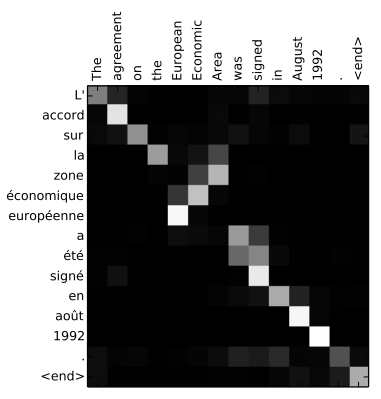
\includegraphics[keepaspectratio,
                   width=.5\paperwidth]{eng_to_french.png}

  {\small Attention Model Interpretability: Visualization of} $\alpha_{ti}$
  \end{center}
\end{frame}


\begin{frame}
  \frametitle{Attention for annotating images}

  \begin{center}
    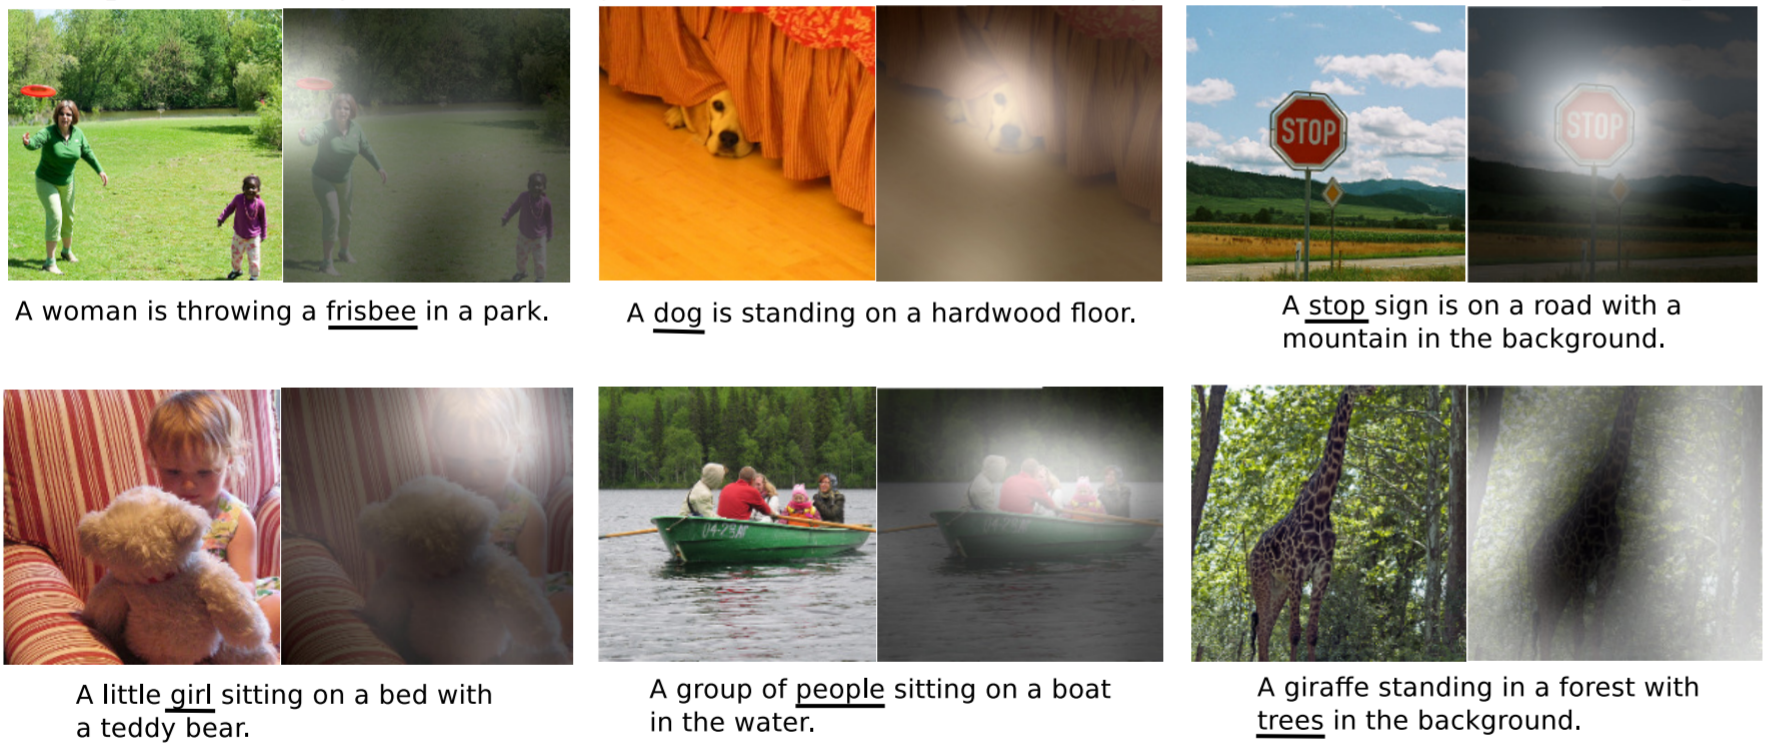
\includegraphics[keepaspectratio,
                   width=.8\paperwidth]{image_attention.png}
  \end{center}

  When generating a word for an image description, the visualization shows which areas of the image the model pays attention to.

  \noindent\rule{8cm}{0.4pt}

  {\small
  {\it Kelvin Xu et al.} Show, attend and tell: neural image caption generation with visual
  attention. 2016}
\end{frame}


\begin{frame}
\frametitle{Vector Similarity Functions}

         $a(h, h^\prime) = h^T h^\prime$ is the scalar (inner) product

         $a(h, h^\prime) = exp(h^T h^\prime)$ — norm becomes SoftMax

         $a(h, h^\prime) = h^T {\color{red}W} h^\prime$ — with the learning parameter matrix $\color{red}{W}$

         $a(h, h^\prime) = {\color{red}w^T} \tanh ({\color{red}U}h + {\color{red}V} h^\prime)$ is additive attention with ${\color{red}w, U, V}$

         \vspace{0.5cm}
         {\bf Linear vector transformations} query, key, value:

    \begin{columns}
      \begin{column}{.6\paperwidth}
        $a(h_i, h^\prime_{t-1}) = ({\color{red}W_k}h_i)^T ({\color{red}W_q}h^\prime_{t-1}) / \sqrt{d}$

        $\alpha_{ti} = \text{SoftMax}_i a(h_i, h^\prime_{t-1})$

        $c_t = \sum\limits_i \alpha_{ti} {\color{red}W_v} h_i $

        ${\color{red}W_q}_{d \times dim(h^\prime)}, {\color{red}W_k}_{d \times dim(h)}, {\color{red}W_v} _{d \times dim(h)}$ — linear neuron weight matrices,
         possible simplification ${\color{red}W_k} \equiv {\color{red}W_v}$
         {\footnotesize
         \noindent\rule{8cm}{0.4pt}

         {\it Dichao Hu.} An introductory survey on attention mechanisms in NLP problems. 2018}
      \end{column}
      \begin{column}{.18\paperwidth}
        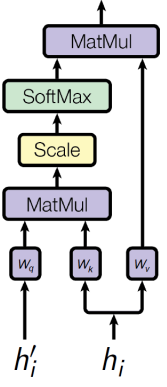
\includegraphics[keepaspectratio,
                         width=.15\paperwidth]{general_attention.png}
      \end{column}
    \end{columns}
\end{frame}

\note{Let's discuss in detail the math inside attention. The first one is Similarity Functions of two vectors. Of course in the simplest case it could be the scalar (inner) product. Also you could use the trainable parameters and our favorite linear transformation layer with non-linear sigmoid function and weights vector.
But the most common procedure is to have query, key, value parameters matrices.}

\begin{frame}
  \frametitle{Attention formula}

  $q$ is the query vector for which we want to calculate the context

  $K = (k_1, \dots, k_n)$ — key vectors compared with the query

  $V = (v_i, \dots, v_n)$ — value vectors forming the context

  $a(k_i, q)$ — score of relevance (similarity) of key $k_i$ to query $q$

  $c$ is the desired context vector relevant to the query

  \pause
  {\small
  \begin{block}{Attention Model}
   This is a 3-layer network that computes a convex combination of $v_i$ values 
   relevant to the query $q$:

   $$ c = Attn(q,K,V) = \sum\limits_i v_i \text{SoftMax}_i a(k_i, q) $$
 \end{block}
 }

  \pause
  $c_t = Attn({\color{red}W_q} h^\prime_{t-1}, {\color{red}W_k} H, {\color{red}W_v} H)$ is the example from the previous slide, where $H = (h_1, \dots, h_n)$ are input vectors, $h^\prime_{t-1}$ is output

  \pause
  Self-attention:

  $c_i = Attn({\color{red}W_q} h_{i}, {\color{red}W_k} H, {\color{red}W_v} H)$ 
  is a special case when $h^\prime \in H$
\end{frame}

\note{In general case we could say, that it is three-layer network, and attention mechanism chooses the best way to store information from the input to the one output vector c. 
And one important case needs to be highlighted here. It is called self-attention.}


\begin{frame}
  \frametitle{Multi-Head Attention}

  {\bf Idea}: $J$ different attention models are jointly trained to highlight various aspects of the input information (for example, parts of speech, syntax, idioms):

  $ c^j = \text{Attn}({\color{red}W^j_q} q, {\color{red}W^j_k} H, {\color{red}W^j_v} H), j = 1, \dots, J$

  \pause
  {\bf Variants} of aggregating the output vector:

  $ c = \frac{1}{J} \sum\limits_{j=1}^J c^j$ — averaging

  $ c = [c^1 \dots c^J]$ — concatenation

  $ c = [c^1 \dots c^J] {\color{red}W}$ — to return to the desired dimension

  \pause
  {\bf Regularization}: to make aspects of attention as different as possible, rows $J \times n$ of matrices $A, \alpha_{ji} = \text{SoftMax}_i a({\color{red}W_k^j}h_i, {\color{red}W_q^j}q)$, decorrelated $(\alpha_{s}^T\alpha_{j} \to 0)$ and sparse $(\alpha_{j}^T\alpha_{j} \to 1)$:
  $$\|AA^T - I \|^2 \to \min\limits_{\{{\color{red}W_k^j}, {\color{red}W_q^j}\}} $$

  \noindent\rule{8cm}{0.4pt}
  \vspace{-0.1cm}

  {\small
  {\it Zhouhan Lin, Y.Bengio et al}. A structured self-attentive sentence embedding. 2017}
\end{frame}


\note{Ok, and the last generalization in this lecture — is multi-head attention. Here you do all the same, but having J different attention models :)}

\begin{frame}
  \frametitle{Not covered in detail in this lecture}

   \begin{itemize}
     \item hierarchical attention (e.g. for classifying documents): words $\in$ sentences $\in$ documents
     \item Graph Attention Network (GAT): multi-class multi-label classification of graph vertices
   \end{itemize}
   \vspace{3cm}

  \noindent\rule{8cm}{0.4pt}

  {\small
  {\it Z.Yang, A.Smola et al.} Hierarchical attention networks for document classification. 2016

  {\it Petar Velickovic et al.} Graph Attention Networks. ICLR-2018}
\end{frame}


{ % all template changes are local to this group.
    \setbeamertemplate{navigation symbols}{}
    \begin{frame}<article:0>[plain]
        \begin{tikzpicture}[remember picture,overlay]
            \node[at=(current page.center)] {
                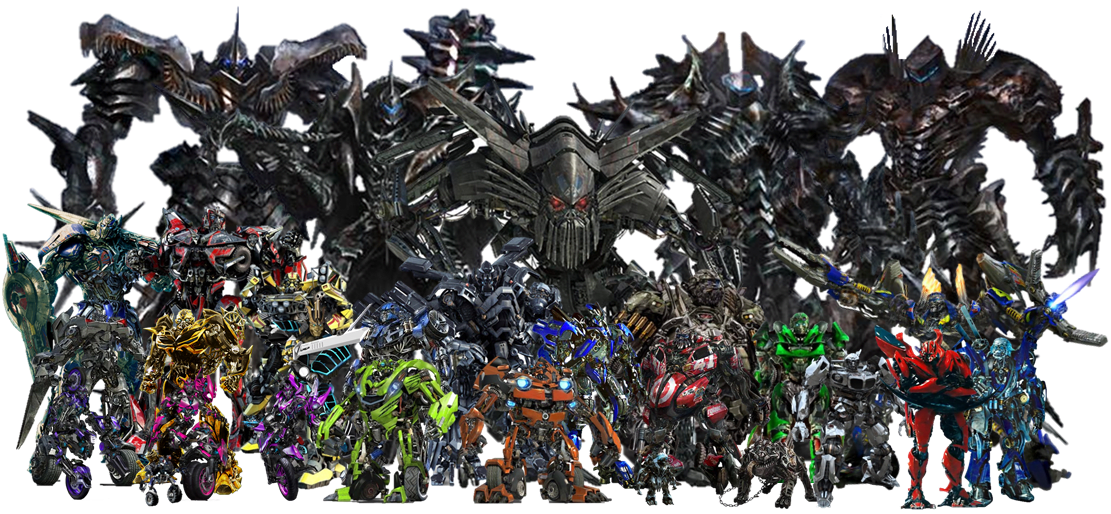
\includegraphics[keepaspectratio,
                                 width=\paperwidth,
                                 height=\paperheight]{many_transformers.png}
            };
        \end{tikzpicture}
     \end{frame}
}

\note{Ok, finally, what is it, who knows?}

\begin{frame}
  \frametitle{Transformer for machine translation}

  Transformer is a neural network architecture based on attention models and fully connected layers, {\bf without RNN}

  \pause
  Scheme of data transformations in machine translation:

  \begin{itemize}
    \item $S = (w_1, \dots, w_n)$ — sentence from words in the input language

          $\downarrow$ trainable or pre-trained word vectorization $\downarrow$
    \item $X = (x_1, \dots, x_n)$ — embeddings of input sentence words

          $\downarrow$ encoder transformer $\downarrow$
    \item $Z = (z_1, \dots, z_n)$ — contextual embeddings

          $\downarrow$ transformer-decoder $\downarrow$
    \item $Y = (y_1, \dots, y_m)$ — embeddings of output sentence words

          $\downarrow$ generation of words from the constructed language model $\downarrow$
    \item $\tilde S = (\tilde w_1, \dots, \tilde w_m)$ — sentence words in target language
  \end{itemize}

  \noindent\rule{8cm}{0.4pt}

  {\small
  {\it Vaswani et al.} (Google) Attention is all you need. 2017}
\end{frame}


\begin{frame}
  \frametitle{Architecture of Transformer Encoder}

    \begin{columns}
      \begin{column}{.2\paperwidth}
        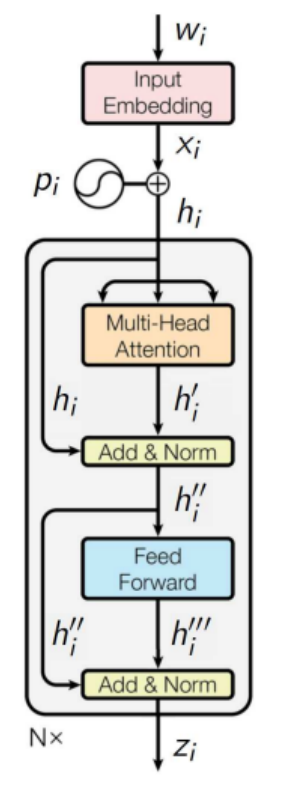
\includegraphics[keepaspectratio,
                         width=.2\paperwidth]{transformer_encoder.png}
      \end{column}
      \begin{column}{.78\paperwidth}
        \begin{enumerate}
          \item position vectors $p_i$ are added: 

          \begin{tabular}{lr}
            \multirow{2}{*}{$h_i = x_i + p_i, \ H = (h_1, \dots, h_n)$} & ${\scriptscriptstyle d = dim\ x_i, p_i, h_i = 512}$ \\
                   & ${\scriptscriptstyle dim\ H = 512 \times n }$
          \end{tabular}

          \pause
          \item multi-head self-attention:

          \begin{tabular}{lr}
            \multirow{3}{*}{$h_i^j = Attn({\color{red}W_q^j} h_{i}, {\color{red} W_k^j} H, {\color{red}W_v^j} H)$} &
            ${\scriptscriptstyle j = 1, \dots, J = 8}$ \\
            &${\scriptscriptstyle dim\ h_i^j = 64}$ \\
            &${\scriptscriptstyle dim\ W_q^j, W_k^j, W_v^j = 64 \times 512}$
          \end{tabular}
          \pause
          \item concatenation:

          \begin{tabular}{lr}
            $h_i^\prime = MH_j(h_i^j) \equiv [h_i^1 \dots h_i^J]$ & ${\scriptscriptstyle dim\ h_i^\prime = 512}$
          \end{tabular}
          \pause
          \item Skip-connection and layer normalization:

          \begin{tabular}{lr}
            $h_i^{\prime\prime} = LN(h_i^\prime + h_i; {\color{red}\mu_1, \sigma_1})$ & ${\scriptscriptstyle dim\ h_i^{\prime\prime}, \mu_1, \sigma_1 = 512}$
          \end{tabular}
          \pause
          \item Fully connected two-layer network FFN:

          \begin{tabular}{lr}
            \multirow{2}{*}{$h_i^{\prime\prime\prime} = {\color{red} W_2} ReLU({\color{red} W_1}h_i^{\prime\prime} + {\color{red} b_1}) + {\color{red} b_2}$} & 
            ${\scriptscriptstyle dim\ W_1 = 2048 \times 512}$ \\
                   & ${\scriptscriptstyle dim\ W_2 = 512 \times 2048}$
          \end{tabular}
          \pause
          \item Skip-connection and layer normalization:

          \begin{tabular}{lr}
            $z_i = LN(h_i^{\prime\prime\prime} + h_i^{\prime\prime}; {\color{red}\mu_2, \sigma_2})$ & ${\scriptscriptstyle dim\ z_i, \mu_2, \sigma_2 = 512}$
          \end{tabular}
        \end{enumerate}
      \end{column}
    \end{columns}
\end{frame}


\begin{frame}
  \frametitle{Additions and remarks}

    \begin{itemize}
      \item a lot of such blocks $N=6, h_i \to \square \to z_i$ are connected in series
      \item calculations can be easily parallelized in $x_i$
      \item it is possible to use pre-trained $x_i$ embeddings
      \item it is possible to learn embeddings $x_i$ of words $w_i \in V$
      \item Layer Normalization (LN), $x, {\color{red}\mu}, {\color{red}\sigma} \in \mathbb{R}^d$
    \end{itemize}

    \begin{align*}
      LN_s(x; {\color{red}\mu}, {\color{red}\sigma}) = {\color{red}\mu_s} + {\color{red}\sigma_s} \frac{x_s - \overline{x}}{\sigma_x} \\
      \overline{x} = \frac{1}{d} \sum\limits_{s=1}^d x_s, \sigma_x^2 = \frac{1}{d} \sum\limits_{s=1}^ d (x_s - \overline{x})
    \end{align*}
\end{frame}

\note{Layer Normalization is quite easy — you train the mean and variance values of components of your vectors}

\begin{frame}
  \frametitle{Positional encoding}

   The positions of the words $i$ are encoded by the vectors $p_i$ so that
   \begin{itemize}
     \item the more $|i-j|$, the more $\|p_i-p_j\|$
     \item number of positions is not limited
   \end{itemize}

   \pause
   \vspace{1cm}
   For example,

   $ c_j = \text{Attn}(q_j, K, V) = \sum_i (v_i + {\color{red}w^v_{i\boxminus j}}) \text{SoftMax}_i a(k_i + {\color{red} w^k_{i\boxminus j}}, q_j), $

   where $i\boxminus j = \max(\min(i-j, \delta), -\delta)$ is the truncated difference, $\delta = 5..16$

   \vspace{1cm}
   \noindent\rule{8cm}{0.4pt}

   {\small
   {\it Shaw, Uszkoreit, Vaswani.} Self-attention with relative position representations. 2018}
\end{frame}

\begin{frame}
  \frametitle{Architecture of Transformer Decoder}

    \begin{columns}
      \begin{column}{.28\paperwidth}
        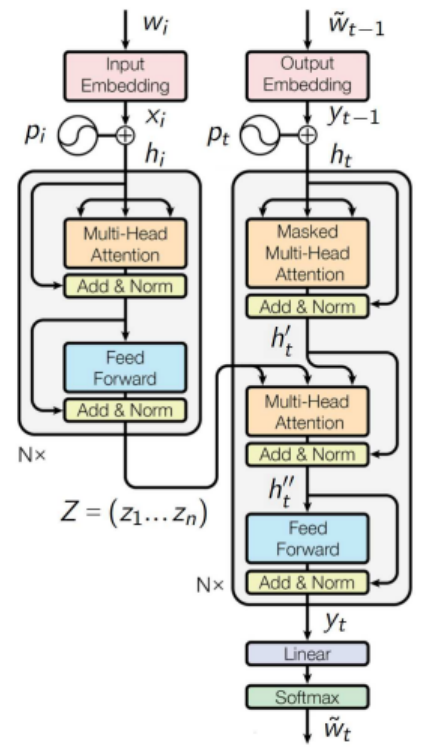
\includegraphics[keepaspectratio,
                         width=.28\paperwidth]{transformer_decoder.png}
      \end{column}
      \begin{column}{.68\paperwidth}
      Autoregressive sequence synthesis

      $y_0 = \left< BOS \right>$ — start symbol embedding;

      \textbf{for all} $t = 1,2,\dots$:
        \begin{enumerate}
          \item masking data ``from the future'':

          $h_t = y_{t-1} + p_t; \ H_t = (h_1, \dots, h_t)$

          \pause
          \item multi-head self-attention:

          $h_t^\prime = {\color{olive} LN_{sc}} \circ MH_j \circ Attn({\color{red}W_q^j} h_{t}, {\color{red} W_k^j} H_t, {\color{red}W_v^j} H_t)$
          \pause
          \item multi-head attention on the Z vectors:

          $h_t^{\prime\prime} = {\color{olive} LN_{sc}} \circ MH_j \circ Attn({\color{red}\tilde W_q^j} h_{t}^\prime, {\color{red}\tilde W_k^j} Z, {\color{red}\tilde W_v^j} Z)$
          \pause
          \item two-layer neural network:

          $y_t = {\color{olive} LN_{sc}} \circ FFN(h_t^{\prime\prime})$
          \pause
          \item linear predictive layer:

          $p(\tilde w|t) = SoftMax_{\tilde w}({\color{red} W_y} y_t + {\color{red} b_y})$

          \pause
          \item generation $\tilde w_t = \arg\max\limits_{\tilde w} p(\tilde w|t)$ \textbf{until} $\tilde w_t \neq \left<EOS\right>$
        \end{enumerate}
      \end{column}
    \end{columns}
\end{frame}

\note{Let's move on to the second part of transformer architecture — the decoder.}

\begin{frame}
\frametitle{Training and validation criteria for machine translation}

  {\bf Criteria for learning} parameters of the neural network $\color{red}{W}$ on the training set of sentences $S$ with translation $\tilde S$:

  $$ \sum\limits_{(S, \tilde S)} \sum\limits_{\tilde w_t \in \tilde S} \ln p(\tilde w_t|t, S, {\color{red}W}) \to \max\limits_W $$

  \pause
  {\bf Criteria for evaluating models} (non-differentiable) based on a sample of pairs of sentences "translation $S$, standard $S_0$":

  BiLingual Evaluation Understudy:

  \begin{align*}
    \text{BLEU} &= \min \left(1, \frac{\sum \text{len}(S)}{\sum \text{len}(S_0)} \right) \times \\
    \underset{(S_0, S)}{\text{mean}}&\left(\prod\limits_{n=1}^4 \frac{\#n\text{-gram from } S, \text{incoming in } S_0}{\#n\text{-gram in } S} \right)^{\frac14}
  \end{align*}
\end{frame}


{ % all template changes are local to this group.
    \setbeamertemplate{navigation symbols}{}
    \begin{frame}<article:0>[plain]
        \begin{tikzpicture}[remember picture,overlay]
            \node[at=(current page.center)] {
                
\includegraphics[keepaspectratio,
                                 width=\paperwidth,
                                 height=\paperheight]{BERT_real.png}
            };
        \end{tikzpicture}
     \end{frame}
}


\begin{frame}
  \frametitle{BERT — Bidirectional Encoder Representations from Transformers}

  The BERT transformer is a decoderless encoder that can be trained to solve a wide range of NLP problems.

  Scheme of data transformations in NLP tasks:

  \begin{itemize}
    \item $S = (w_1, \dots, w_n)$ — sentence from words in the input language

          $\downarrow$ learning embeddings with transformer $\downarrow$
    \item $X = (x_1, \dots, x_n)$ — embeddings of input sentence words

          $\downarrow$ encoder transformer $\downarrow$
    \item $Z = (z_1, \dots, z_n)$ — contextual embeddings

          $\downarrow$ additional training for a specific task $\downarrow$
    \item $Y$ - output text / markup / classification, etc.
  \end{itemize}

  \noindent\rule{8cm}{0.4pt}

  {\footnotesize
  {\it Jacob Devlin, Ming-Wei Chang, Kenton Lee, Kristina Toutanova} (Google AI Language)
  BERT: pre-training of deep bidirectional transformers for language understanding. 2019.}
\end{frame}


\begin{frame}
  \frametitle{MLM (masked language modeling) criterion for BERT training}

  The masked language modeling criterion is built automatically from texts (self-supervised learning):

  $$ \sum\limits_{S} \sum\limits_{ i \in M(S)} \ln p(w_i|i, S, {\color{red}W}) \to \max\limits_W, $$

  where $M(S)$ is a subset of masked tokens from $S$,

  $$ p(w|i, S, {\color{red}W}) = \underset{w \in V}{\text{SoftMax}}({\color{red}W_z}z_i(S, {\color{red}W_T}) + {\color{red}b_z})$$

  is a language model that predicts the $i$-th sentence token $S$, $z_i(S, {\color{red}W_T})$ is the contextual embedding of the $i$-th sentence token $S$ at the output of the transformer with parameters ${\color{red}W_T}$,

  ${\color{red}W}$ — all transformer and language model parameters
\end{frame}


\begin{frame}
  \frametitle{NSP (next sentence prediction) criterion for BERT training}

  The criterion for predicting the relationship between NSP sentences is built automatically from texts (self-supervised learning):

  $$ \sum\limits_{(S, S^\prime)} \ln p\left(y_{SS^\prime}|S, S^\prime, {\color{red}W}\right) \to \max\limits_W, $$

  where $y_{SS^\prime} = $ [$S$ followed by $S^\prime$] is the binary classification of a pair of sentences,

  $$ p(y|S, S^\prime, {\color{red}W}) = \underset{y \in \{0,1\}}{\text{SoftMax}}\left({\color {red}W_y} \tanh({\color{red}W_s}z_0(S, S^\prime, {\color{red}W_T}) + {\color{red}b_s}) + {\color{red}b_y}\right)$$

  — probabilistic classification model for pairs $(S, S^\prime)$, $z_0(S, S^\prime, {\color{red}W_T})$ — contextual embedding of token $\left<\text{CLS}\right>$ for a sentence pair written as $\left<\text{CLS}\right> S \left<\text{SEP}\right> S^\prime \left<\text{SEP}\right>$
\end{frame}


\begin{frame}
  \frametitle{A few more notes about transformers}

  \begin{itemize}
    \item Fine-tuning: model $f(Z(S, {\color{red}W_T}), {\color{red}W_f})$, sample $\{S\}$ and criterion $\mathcal{L}(S, f) \to \max$
    \item Multi-task learning: for additional training on a set of tasks $\{t\}$, models $f_t(Z(S, {\color{red}W_T}), {\color{red}W_f})$, samples $\{S\}_t$ and sum of criteria $ \sum_t \lambda_t \sum_S \mathcal{L}_t(S, f_t) \to \max $
    \item GLUE, SuperGLUE, Russian SuperGLUE — sets of test problems for understanding natural language
    \item Transformers are usually built not on words, but on tokens received by BPE (Byte-Pair Encoding) or WordPiece
    \pause
    \item First transformer: $N = 6, d = 512, J = 8$, weights 65M
    \item $\text{BERT}_{\text{BASE}}$, GPT-1: $N = 12, d = 768, J = 12$, weights 110M
    \item $\text{BERT}_{\text{LARGE}}$, GPT-2: $N = 24, d = 1024, J = 16$, weights 340M-1000M
    \pause
    \item GPT-3: weights 175 billion
    \item Gopher (DeepMind): 280 billion
    \item Turing-Megatron (Microsoft + Nvidia): 530 billion
  \end{itemize}
\end{frame}


\begin{frame}
  \frametitle{Summary}
  \begin{itemize}
    \item Attention models were first built into RNNs or CNNs, but they turned out to be self-sufficient
    \item Based on them, the Transformer architecture was developed, various variants of which (BERT, GPT-3, XLNet, ELECTRA, etc.) are currently SotA in natural language processing tasks, and not only
    \item Multi-head self-attention (MHSA) has been proven to be equivalent to a convolutional network [Cordonnier, 2020]
  \end{itemize}

  \noindent\rule{8cm}{0.4pt}

  {\footnotesize
  {\it Vaswani et al.} Attention is all you need. 2017.

  {\it Dichao Hu.} An Introductory Survey on Attention Mechanisms in NLP Problems. 2018.

  {\it Xipeng Qiu et al.} Pre-trained models for natural language processing: A survey. 2020.

  {\it Cordonnier et al.} On the relationship between self-attention and convolutional layers. 2020}
\end{frame}


\begin{frame}
What else can you see?
   \begin{itemize}
     \item GPT-3 on wikipedia: \href{https://en.wikipedia.org/wiki/GPT-3}{https://en.wikipedia.org/wiki/GPT-3}
     \item Grigory Sapunov \href{https://www.youtube.com/watch?v=8dN6ZVnDArk&t}{about transformers in 2021 (in Russian)}
     \item Nikolai Grigoriev (SE @ Deepmind) \href{https://www.youtube.com/watch?v=8Q-a6-P6Eyo}{about history and modern language models}, February 14, 2022
     \item \href{https://disk.yandex.ru/d/knoQ44wLmGDwwQ}{Seminar of WMC Euler and MCS on formalization of mathematical proofs in Lean and deep learning (in Russian)}
   \end{itemize}
\end{frame}

\end{document}
